\documentclass[a4j,multicol,8pt]{jarticle}
%\documentclass[a4j,twocolumn,8pt]{jarticle}
\usepackage[top=10truemm,bottom=10truemm,left=10truemm,right=10truemm]{geometry}
\usepackage[dvipdfmx]{graphicx}
\usepackage{url}
\usepackage{here}
 \usepackage{multicol}
\renewcommand{\figurename}{Fig.}
\newcommand{\Figref}[1]{Fig~\ref{#1}}
\setlength\textfloatsep{0pt} % 本文と図の間の余白
\setlength\abovecaptionskip{1pt} % 図とキャプションの余白
\usepackage{titlesec}
\titleformat*{\section}{\large\bfseries}
% あがき
%\renewcommand{\baselinestretch}{0.75}
%\setlength\abovecaptionskip{1truemm}
%\setlength\belowcaptionskip{1truemm}
\makeatletter
%\def\section{\@startsection {section}{1}{\z@}{-2.5ex plus -1ex minus -.2ex}{2.5 ex plus .2ex}{\Large\bf}}
%\def\subsection{\@startsection {subsection}{1}{\z@}{0.5ex}{0.5 ex}{\large\bf}}
%\def\subsection{\@startsection {subsection}{1}{\z@}{-1.0ex plus -1ex minus -.1ex}{3.0 ex plus .2ex}{\Large\bf}}
%\def\subsubsection{\@startsection {subsubsection}{1}{\z@}{-2.5ex plus -1ex minus -.2ex}{.3 ex plus .2ex}{\large \bf $\spadesuit$ }}
\@dblfptop 0pt
\makeatother
%\makeatletter
%  \renewcomand{\section}{
%    \@startsection{section}{1}{\z@}
%    {0.4\Cvs}{0.1\Cvs}
%    {\nomalfont\large\headfont\raggedright}}
%\makeatother

\begin{document}
\pagestyle{empty} 
\title{\Large Numerical experiments of giant planet surface flows  \\
produced by forcings representing thunderstorms
}
%\title{\Large 
%雷雲を想定した強制により生じる巨大惑星表層流の数値計算
%}

\author{\large Ryoma Suzuki (Planetary and Space Group)}
%\author{\large 鈴木 綾馬 (惑星宇宙グループ)}
\date{}
\maketitle
\begin{multicols}{2}
\vspace{-0.2zh}
\section{Introduction}
%\section{はじめに}
\vspace{-0.8zh}
%
It is known that the surfaces of giant planets have
the banded structure consisting of eqatorial jets with wide latitudinal widths,
mid-latitude jets with a narrow latitudinal widths, and
the vortex structure in the polar regions.
%巨大惑星表層には,
%赤道域における緯度幅の広いジェットや
%中緯度域における緯度幅の狭いジェットから成る帯状構造,
%極域における渦構造が存在することが知られている.
Large-scale structures such as bands and polar vortices
can be formed from small-scale turbulence in the atmospheres
due to the inverse cascade effect (Vallis 2017).
Thunderstorms are considered to be
a candidate for causing such small-scale turbulence (e.g. Ingersoll et al., 2000).
%
%帯状構造や極渦のような
%大規模構造はエネルギーの逆カスケード効果(\cite{Vallis2017})によって,
%大気中の小規模乱流から形成される可能性がある.
%このような小規模乱流を
%引き起こす候補として,
%雷雲が考えられる(\cite{Gierasch2000}, \cite{Ingersoll2000}).
%%
%
Showman (2007) and Brueshaber et al. (2019) restricted the
computational domain to a part of the sphere and
calculated in the framework of the shallow water equations
with the mass forcing representing thunderstorms.
%\cite{Showman2007}, \cite{Brueshaber2019} は
%この雷雲を想定した質量強制を加えた浅水実験を
%球面の一部の領域で行った.
%
%
%
Showman (2007) and Brueshaber et al. (2019) restricted the
computational domain to a part of the sphere and
calculated in the framework of the shallow water equations
with the mass forcing representing thunderstorms.
%\cite{Showman2007}, \cite{Brueshaber2019} は
%この雷雲を想定した質量強制を加えた浅水実験を
%球面の一部の領域で行った.
%
%
Showman (2007) restricted the computational domain to the latitude range of
$0^\circ - 70^\circ$ and the longitude range of $0^\circ - 120^\circ$,
and the results showed the formation of the banded structures.
%\cite{Showman2007} は緯度$0^\circ - 70^\circ$,経度$0^\circ - 120^\circ$ の領域を計算した結果,
%帯状構造が形成されることがわかった.
%
Brueshaber et al. (2019) found the polar vortex structures were formed
in the computational domain from latitude $60^\circ$ to high latitude
%\cite{Brueshaber2019} は緯度$60^\circ$ より高緯度の極域を計算し,
%極渦が形成されることがわかった.
%
In addition, their results showed
that the number and size of polar vortices,
the sign of vorticity significantly depend on
the value of Burger number (dimensionless number written
by a ratio of deformation radius to planetary radius).
%また,極渦の数や大きさ,低気圧性・高気圧性といった特徴は
%Burger 数(変形半径と惑星半径の比で書かれる無次元量) の値に
%強く依存することがわかった.
%
However, their computational domain is only a part of the sphere.
It is necessary to confirm their results by calculating on the global domain.
%しかし,どちらの先行研究も領域計算であり,
%全球計算を行い,彼らの結果を確かめる必要がある.
Since the structure of jets and vortices may change due to momentum transport from
outside the restricted computational domain.
%なぜなら,先行研究では考慮されていない
%計算領域外からの運動量輸送などにより,
%計算で得られたジェットや
%渦の構造が変化する可能性があるからである.
%
The purpose of this study is to perform
wheter the jet and polar vortex structures seen on giant planets are
formed by the mass forcing representing thunderstorms.
%本研究の目的は雷雲を想定して与えた質量強制による
%数値実験を全球で行い,雷雲による強制により,
%巨大惑星で見られる帯状構造と極渦が形成されるのかを調べることである
%
Then, compare the global calculation results with the results of previous studies
and consider the validity of the results obtained by domain calculation.
%加えて,それらの構造を先行研究で得られた結果と比較し,
%領域計算で得られた結果の妥当性を調べる.
\vspace{-2zh}
\section{Model and experimental settings}
%\section{モデル, 実験設定}
\vspace{-0.8zh}
The model of this study uses the Hierarchical Spectral Models for GFD (SPMODEL; Takehiro et al. 2006, Takehiro et al. 2013).
%
The used equations are a 1.5-layer shallow water equations
with the mass forcing representing thunderstorms.
%本研究は地球流体電脳倶楽部の階層的地球スペクトルモデル集
%(SPMODEL; \cite{spmodel2006}, \cite{spmodel2013})を用い,
%雷雲を想定した質量強制を加えた1.5層浅水系全球計算を行う.
%
\vspace{-2zh}
\section{Results}
%\section{結果}
\vspace{-0.8zh}
In the standard experimetal results,
the banded structure and
the polar vortex structure were formed.
%標準実験では帯状構造と渦構造が形成した.
%
%
It was also found that the structures remained almost unchanged
even if the positive / negative
ratio of the mass forcing and the spatial size were varied.
%質量強制の正負の割合や,
%空間的大きさを変更した実験を行ったが,
%帯状構造や極渦の構造はほとんど変化しなかった.
%
%
The characteristics of the polar vortex were
found to depend on the value of Burger number:
when the Burger number is small,
small multiple vortices are formed, as observed Jupiter,
and as the Burger number increases,
a single cyclonic vortex is formed, observed on Saturn, Uranus, and Neptune (Fig.1).
%また,極渦の特徴はBurger 数の値に依存することがわかった.
%Burger 数が小さい場合,木星で観測されるような
%比較的小さな複数の渦が形成し,
%Burger 数が大きくなるにつれて,
%土星,天王星,海王星で
%観測されている単一の低気圧性渦が形成する.
\vspace{-2zh}
\section{Conclusion}
%\section{まとめ}
\vspace{-0.8zh}
The banded structures and the polar cortex structures were 
formed in several experiments.
These results are consistent with the results of Showman (2007) and Brueshaber et al. (2019).
%これらの結果は,\cite{Showman2007}, \cite{Brueshaber2019} で
%得られた結果と整合的である.
%
Moreover, the results of the standard experiment show that
the zonal wind speed of the equatorial jet is
about 10 times larger than that of Showman (2007).
%ただし,標準実験で得られた計算結果では
%赤道域でのジェットの風速が\cite{Showman2007} の結果に比べて,
%約10倍大きい.
%
The result possibly suggests that the existence of polar reions and/or opposite hemisphere,
which was not considered in Showman (2007), affect the strength of the jet.
%この結果は\cite{Showman2007} では考慮されていない
%極域あるいは反対半球の存在が
%ジェットの強度に影響を与える可能性を示唆している.
%
\end{multicols}
\begin{figure*}[b]
  \begin{center}
  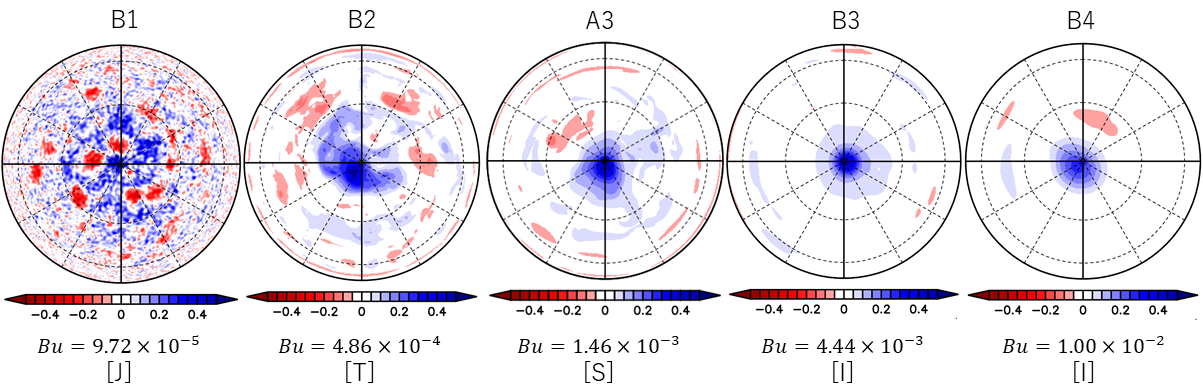
\includegraphics[width=11cm]{./fig/case1_nonqv_a.png}
  \caption{\footnotesize{Nondimensional potential vorticity as a funtion of Burger number.
}}
  \label{case1:nonqv_a}
  \end{center}
\end{figure*}
\end{document}

